\subsection{Kiểm thử API với SwaggerUI}

Sau khi hoàn tất kiểm thử đơn vị, nhóm tiến hành kiểm thử tầng API để xác minh khả năng giao tiếp giữa các thành phần và tính đúng đắn của dữ liệu trả về thực tế. Trong dự án này, nhóm sử dụng Swagger UI (OpenAPI 3.0) làm công cụ chính để thực hiện kiểm thử thủ công trực tiếp trên từng Microservice.

\subsubsection{Thiết lập môi trường kiểm thử}
Nhóm cấu hình thư viện springdoc-openapi cho tất cả các dịch vụ, cho phép truy cập giao diện kiểm thử tại đường dẫn: \texttt{http://localhost:[port]/swagger-ui/index.html} hoặc địa chỉ IP 57.155.x.xxx của Azure khi triển khai thực tế.

Các bước thực hiện kiểm thử tiêu biểu bao gồm:
\begin{itemize}
    \item Xác thực: Đối với các Endpoint yêu cầu bảo mật, nhóm thực hiện đăng nhập để lấy mã \texttt{JWT Access Token}, sau đó sử dụng tính năng "Authorize" trên Swagger để gắn token vào header của mọi yêu cầu tiếp theo.
    \item Thực thi: Truyền các tham số đầu vào như path variable hay query parameter hoặc cấu trúc JSON của request body trực tiếp trên giao diện và nhấn "Execute".
    \item Kiểm chứng: Nhóm đánh giá kết quả dựa trên các tiêu chí:
    \begin{itemize}
        \item Mã trạng thái HTTP phù hợp.
        \item Cấu trúc dữ liệu JSON trả về đúng tên trường và định dạng dữ liệu.
        \item Sự thay đổi trạng thái của hệ thống (ví dụ: dữ liệu được lưu vào Database hoặc tin nhắn được gửi đi thành công).
    \end{itemize}
\end{itemize}

\subsubsection{Phạm vi và kịch bản tiêu biểu}

Để khẳng định tính sẵn sàng của hệ thống, nhóm tập trung thực hiện các kịch bản kiểm thử luồng nghiệp vụ chuẩn trực tiếp trên giao diện Swagger UI. Đây là giai đoạn quan trọng nhằm kiểm chứng sự phối hợp đồng bộ giữa các Microservices độc lập thông qua cơ chế gọi API trực tiếp và truyền tin bất đồng bộ.

\textbf{A. Kiểm thử tích hợp các luồng chức năng cốt lõi}

Nhóm thực hiện các chuỗi thao tác liên tục để đảm bảo luồng dữ liệu không bị ngắt quãng giữa các tầng xử lý:

\begin{itemize}
    \item Luồng xác thực và định danh: Thực hiện đăng nhập để nhận JWT Token. Sau đó, sử dụng token này để kiểm tra quyền truy cập vào các tài nguyên bảo mật, đảm bảo tính năng phân quyền hoạt động đúng như thiết kế.
    \item Luồng truy vấn và lựa chọn sản phẩm: Kiểm tra các Endpoint lấy danh sách cây cảnh với các bộ lọc phức tạp. Xác nhận dữ liệu JSON trả về khớp hoàn toàn với cấu trúc DTO, đảm bảo đầy đủ thông tin về biến thể và hình ảnh sản phẩm.
    \item Luồng đặt hàng hoàn chỉnh: Đây là kịch bản phức tạp nhất, đi từ việc thêm sản phẩm vào giỏ hàng, tính toán giá trị đến khi khởi tạo quy trình thanh toán thông qua orchestration service.
\end{itemize}

\begin{figure}[H]
\centering
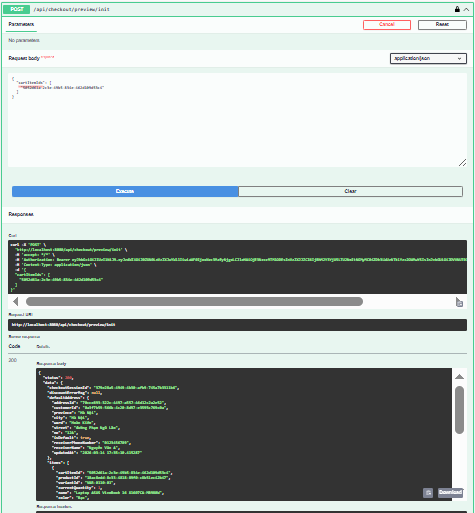
\includegraphics[width=0.9\linewidth]{images/chap8/api-success-2.PNG}
\vspace{0.7cm}
\caption{Thực thi thành công API lấy thông tin đặt hàng trên Swagger UI}
\label{fig:swagger-checkout}
\end{figure}

Giao diện Swagger hiển thị ở hình \ref{fig:swagger-checkout} kết quả khởi tạo quy trình thanh toán thành công với mã phản hồi 200. Hệ thống đã tiếp nhận danh sách các mã mục giỏ hàng và trả về thông tin chi tiết về địa chỉ mặc định cùng danh sách sản phẩm chờ xác nhận.

\textbf{B. Xác minh phản hồi và tính nhất quán dữ liệu}

Thông qua việc quan sát kết quả trực tiếp, nhóm tập trung đánh giá hai yếu tố then chốt là tính chính xác của dữ liệu và cơ chế báo lỗi hệ thống:

\begin{itemize}
    \item Nhóm thực hiện kiểm chứng các thông tin định lượng quan trọng như tổng giá trị giỏ hàng sau khi áp dụng mã giảm giá tại cart, hoặc trạng thái tồn kho thực tế tại product. Các dữ liệu này phải phản hồi chính xác tuyệt đối với mã trạng thái \texttt{200 OK}, đảm bảo sự đồng nhất giữa logic xử lý tại Backend và dữ liệu hiển thị cho người dùng.
    \item Thông báo trạng thái hệ thống: Backend được thiết lập cơ chế xử lý ngoại lệ tập trung. Trong các tình huống phát sinh lỗi logic hoặc sai lệch dữ liệu ngoài kịch bản chuẩn, hệ thống được cấu hình để phản hồi mã \texttt{500 Internal Server Error} kèm theo thông báo mô tả nguyên nhân cụ thể, giúp đội ngũ phát triển dễ dàng theo dõi và khắc phục sự cố.
\end{itemize}

\begin{figure}[H]
\centering
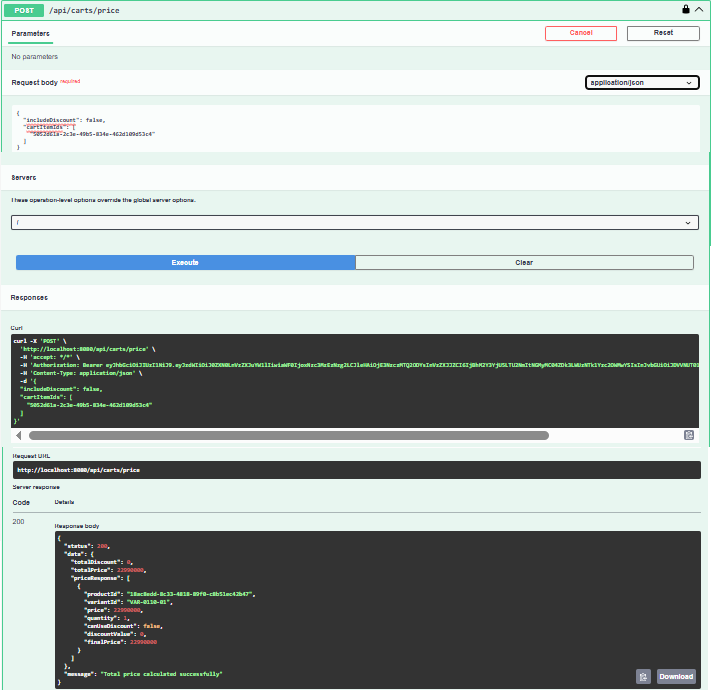
\includegraphics[width=0.9\linewidth]{images/chap8/api-success-3.PNG}
\vspace{0.7cm}
\caption{Minh họa phản hồi kết quả tính toán giá trị giỏ hàng trên Cart Service}
\label{fig:swagger-cart}
\end{figure}

Hình \ref{fig:swagger-cart} minh họa kết quả kiểm thử API tính toán giá trị giỏ hàng thực tế sau khi áp dụng các quy tắc giảm giá. Dữ liệu phản hồi với mã trạng thái \texttt{200 OK} đã xác nhận tính chính xác của tổng số tiền cần thanh toán và các mức chiết khấu đi kèm, đảm bảo logic nghiệp vụ tại cart service vận hành hoàn toàn khớp với các kịch bản kiểm thử đơn vị đã thiết lập trước đó.

Toàn bộ các API được kiểm thử thủ công đều phản hồi đúng theo đặc tả kỹ thuật ban đầu. Việc sử dụng Swagger UI không chỉ giúp nhóm phát hiện sớm các lỗi về định dạng dữ liệu mà còn đóng vai trò là tài liệu hướng dẫn trực quan cho việc tích hợp với giao diện sau này.

